\documentclass[11pt,a4paper]{article}

% ==================== ПАКЕТЫ ====================
\usepackage[utf8]{inputenc}
\usepackage[T2A]{fontenc}
\usepackage[russian]{babel}
\usepackage[left=1.8cm, right=1.8cm, top=2.5cm, bottom=2cm]{geometry}
\usepackage{amsmath, amssymb}
\usepackage{graphicx}
\usepackage[dvipsnames,svgnames,table]{xcolor}
\usepackage[most]{tcolorbox}
\usepackage{tikz}
\usepackage{booktabs}
\usepackage{hyperref}
\usepackage{fancyhdr}
\usepackage{enumitem}
\usepackage{float}
\usepackage{titlesec}
\usepackage{array}
\usepackage{longtable}
\usepackage{multirow}
\usepackage{caption}
\usepackage{eso-pic}
\usepackage{tabularx}
\usepackage{ragged2e}
\usepackage{setspace}
\usepackage{listings}

\usetikzlibrary{arrows.meta, positioning, shapes.geometric, calc, fit, backgrounds}

\linespread{1.15}

% ==================== ЦВЕТА ====================
\definecolor{pastelblue}{RGB}{163,210,237}
\definecolor{pastelgreen}{RGB}{152,225,172}
\definecolor{pastelyellow}{RGB}{255,243,196}
\definecolor{pastelorange}{RGB}{255,210,170}
\definecolor{pastelpurple}{RGB}{200,170,220}
\definecolor{pastelred}{RGB}{250,180,185}
\definecolor{pastelteal}{RGB}{170,215,220}
\definecolor{darkblue}{RGB}{40,60,100}
\definecolor{accentblue}{RGB}{70,130,180}
\definecolor{softgray}{RGB}{140,140,140}
\definecolor{sectioncolor}{RGB}{50,50,50}
\definecolor{mvideored}{RGB}{227,30,36}
\definecolor{mvideodark}{RGB}{26,26,46}

\definecolor{CUSky}{RGB}{220,234,245}
\definecolor{CURose}{RGB}{246,226,228}
\definecolor{CUSand}{RGB}{245,238,220}
\definecolor{CUMint}{RGB}{224,240,234}
\definecolor{CULilac}{RGB}{236,230,248}

\newcolumntype{Y}{>{\RaggedRight\arraybackslash}X}

\newcommand{\cblue}[1]{\textcolor{accentblue}{\textbf{#1}}}
\newcommand{\cgreen}[1]{\textcolor{pastelgreen!60!black}{\textbf{#1}}}
\newcommand{\corange}[1]{\textcolor{pastelorange!70!black}{\textbf{#1}}}
\newcommand{\cpurple}[1]{\textcolor{pastelpurple!60!black}{\textbf{#1}}}
\newcommand{\cteal}[1]{\textcolor{pastelteal!60!black}{\textbf{#1}}}
\newcommand{\cred}[1]{\textcolor{mvideored}{\textbf{#1}}}
\newcommand{\keyword}[1]{\textcolor{accentblue}{\textbf{#1}}}
\newcommand{\hlblue}[1]{\colorbox{pastelblue!25}{\textcolor{sectioncolor}{\strut #1}}}
\newcommand{\hlgreen}[1]{\colorbox{pastelgreen!25}{\textcolor{sectioncolor}{\strut #1}}}
\newcommand{\hlred}[1]{\colorbox{pastelred!25}{\textcolor{sectioncolor}{\strut #1}}}

\hypersetup{
    colorlinks=true,
    linkcolor=accentblue,
    urlcolor=mvideored,
    citecolor=accentblue,
    unicode=true,
    pdftitle={Документация М.Видео NER Search},
}

\pagestyle{fancy}
\fancyhf{}
\renewcommand{\headrulewidth}{0.4pt}
\fancyhead[L]{\small\textcolor{softgray}{М.Видео --- Интеллектуальный поиск (NER)}}
\fancyhead[R]{\small\textcolor{softgray}{Буткемп ЦУ 2026}}
\fancyfoot[C]{\thepage}
\setlength{\headheight}{14pt}

\titleformat{\section}
    {\Large\bfseries\color{sectioncolor}}
    {\thesection.}{0.5em}{}[\vspace{2pt}\textcolor{mvideored}{\hrule height 1.5pt}]
\titleformat{\subsection}
    {\large\bfseries\color{sectioncolor}}
    {\thesubsection.}{0.5em}{}

\newtcolorbox{definitionbox}[1][]{
    enhanced, breakable,
    colback=pastelblue!12, colframe=pastelblue!60!black,
    coltitle=white, fonttitle=\bfseries,
    title={#1},
    attach boxed title to top left={yshift=-2mm, xshift=4mm},
    boxed title style={colback=pastelblue!60!black, sharp corners},
    sharp corners, boxrule=0.8pt,
    left=6pt, right=6pt, top=6pt, bottom=6pt,
}

\newtcolorbox{remarkbox}[1][]{
    enhanced, breakable,
    colback=pastelyellow!20, colframe=pastelorange!70!black,
    coltitle=white, fonttitle=\bfseries,
    title={#1},
    attach boxed title to top left={yshift=-2mm, xshift=4mm},
    boxed title style={colback=pastelorange!70!black, sharp corners},
    sharp corners, boxrule=0.8pt,
    left=6pt, right=6pt, top=6pt, bottom=6pt,
}

\newtcolorbox{importantbox}[1][]{
    enhanced, breakable,
    colback=pastelred!12, colframe=mvideored,
    coltitle=white, fonttitle=\bfseries,
    title={#1},
    attach boxed title to top left={yshift=-2mm, xshift=4mm},
    boxed title style={colback=mvideored, sharp corners},
    sharp corners, boxrule=0.8pt,
    left=6pt, right=6pt, top=6pt, bottom=6pt,
}

\newtcolorbox{goalbox}[1][]{
    enhanced, breakable,
    colback=pastelgreen!12, colframe=pastelgreen!60!black,
    coltitle=white, fonttitle=\bfseries,
    title={#1},
    attach boxed title to top left={yshift=-2mm, xshift=4mm},
    boxed title style={colback=pastelgreen!60!black, sharp corners},
    sharp corners, boxrule=0.8pt,
    left=6pt, right=6pt, top=6pt, bottom=6pt,
}

\newtcolorbox{purplebox}[1][]{
    enhanced, breakable,
    colback=pastelpurple!12, colframe=pastelpurple!60!black,
    coltitle=white, fonttitle=\bfseries,
    title={#1},
    attach boxed title to top left={yshift=-2mm, xshift=4mm},
    boxed title style={colback=pastelpurple!60!black, sharp corners},
    sharp corners, boxrule=0.8pt,
    left=6pt, right=6pt, top=6pt, bottom=6pt,
}

\newtcolorbox{infobox}{
    enhanced, breakable,
    colback=pastelblue!6, colframe=pastelblue!30,
    boxrule=0.4pt, sharp corners,
    left=10pt, right=10pt, top=10pt, bottom=10pt,
}

\newtcolorbox{summarybox}{
    enhanced, breakable,
    colback=CUSky, colframe=CUSky,
    boxrule=0pt, arc=4mm,
    borderline west={1.5mm}{0pt}{accentblue},
    left=5mm, right=5mm, top=3mm, bottom=3mm,
}

\setlist[enumerate,1]{label=\arabic*., leftmargin=*, itemsep=0.35em, topsep=0.4em}
\graphicspath{{figures/}{../figures/}}

\begin{document}

% ==================== ТИТУЛ ====================
\thispagestyle{empty}
\begin{tikzpicture}[remember picture, overlay]
    \fill[white] (current page.south west) rectangle (current page.north east);
    \fill[mvideored!10] ([yshift=-5.5cm]current page.north west) rectangle (current page.north east);
    \draw[mvideored!35, line width=0.5pt] ([yshift=-5.5cm]current page.north west) -- ([yshift=-5.5cm]current page.north east);
    \fill[pastelblue!10] (current page.south west) rectangle ([yshift=3.2cm]current page.south east);
    \fill[pastelred!15] ([xshift=-1.2cm,yshift=-1.2cm]current page.north east) circle (2.8cm);
    \fill[pastelgreen!12] ([xshift=1.8cm,yshift=2.1cm]current page.south west) circle (3.0cm);

    \node[anchor=center, font=\Large\bfseries\color{sectioncolor}] at ([yshift=-2.3cm]current page.north) {Центральный Университет};
    \node[anchor=center, font=\large\color{softgray}] at ([yshift=-3.5cm]current page.north) {Буткемп $\cdot$ кейс М.Видео $\cdot$ NLP / NER};
    \node[anchor=center, font=\fontsize{24}{30}\selectfont\bfseries\color{mvideodark}] at ([yshift=2.8cm]current page.center) {ИНТЕЛЛЕКТУАЛЬНЫЙ ПОИСК};
    \draw[mvideored!50, line width=0.7pt] ([xshift=4.2cm, yshift=1.7cm]current page.center) -- ([xshift=-4.2cm, yshift=1.7cm]current page.center);
    \node[anchor=center, font=\fontsize{16}{20}\selectfont\color{mvideored}] at ([yshift=0.9cm]current page.center) {ДОКУМЕНТАЦИЯ РЕШЕНИЯ};
    \node[anchor=center, font=\normalsize\color{sectioncolor}] at ([yshift=-0.3cm]current page.center) {Извлечение сущностей из поисковых запросов};

    \node[anchor=center] at ([yshift=-2.8cm]current page.center) {%
        \begin{tikzpicture}
            \node[fill=mvideored!8, rounded corners=6pt, inner sep=10pt, draw=mvideored!35, line width=0.5pt] {%
                \begin{minipage}{11cm}\centering
                \textcolor{accentblue}{\textbf{Репозиторий:}} \url{https://github.com/xWooshieL/mvideo-ner-search}\\[3pt]
                \textcolor{accentblue}{\textbf{Дата:}} 18 июля 2026\\[3pt]
                \textcolor{accentblue}{\textbf{SLA:}} ответ сервиса $<$ 100~мс (JSON)
                \end{minipage}
            };
        \end{tikzpicture}
    };

    \node[anchor=south, font=\footnotesize\color{softgray}] at ([yshift=1cm]current page.south) {%
        Буткемп $\;\cdot\;$ М.Видео $\;\cdot\;$ Центральный Университет $\;\cdot\;$ 2026
    };
\end{tikzpicture}

\newpage
\tableofcontents
\newpage

\section*{Терминология и сокращения}
\addcontentsline{toc}{section}{Терминология и сокращения}
\begin{infobox}
\begin{enumerate}[leftmargin=*, itemsep=4pt]
    \item \keyword{NER} --- Named Entity Recognition, распознавание именованных сущностей.
    \item \keyword{BIO} --- схема разметки токенов: Begin / Inside / Outside.
    \item \keyword{SKU} --- Stock Keeping Unit, единица товарного учёта.
    \item \keyword{CRF} --- Conditional Random Field, модель последовательности для NER.
    \item \keyword{TF-IDF} --- Term Frequency -- Inverse Document Frequency.
    \item \keyword{Weak supervision} --- автоматическая разметка по словарям и правилам.
    \item \keyword{YML} --- Yandex Market Language, формат товарного каталога.
    \item \keyword{SLA} --- целевое время ответа сервиса ($<$ 100~мс).
\end{enumerate}
\end{infobox}

\newpage

\section{Введение}

\subsection{О кейсе}

Поисковая система М.Видео должна \cred{определять категорию, бренд и характеристики} товара в пользовательском запросе. Ошибки разбора ведут к нерелевантной выдаче и потере конверсии.

\begin{goalbox}[Цель буткемпа]
Построить алгоритм/сервис, который на вход получает строку-запрос и менее чем за \hlred{100~мс} возвращает структурированный JSON с извлечёнными фактами.
\end{goalbox}

\subsection{Критерий успеха}

\begin{enumerate}
    \item Словари, модели и/или сервис на Python.
    \item Структурированный JSON: сущности, бренд, категория, атрибуты.
    \item Latency p95 существенно ниже 100~мс на CPU.
    \item Метрики качества: Accuracy, Precision, Recall, F1.
\end{enumerate}

\subsection{Дорожная карта буткемпа}

\begin{center}
\begin{tikzpicture}[
    box/.style={rectangle, draw=mvideored!50, fill=mvideored!6, rounded corners=3pt,
                minimum height=1.1cm, text width=2.1cm, align=center, font=\scriptsize\bfseries},
    arr/.style={-{Stealth}, thick, softgray}]
    \node[box] (a) at (0,0) {01\\Погружение};
    \node[box] (b) at (3.0,0) {02\\Исследование};
    \node[box] (c) at (6.0,0) {03\\Прототип};
    \node[box] (d) at (9.0,0) {04\\Упаковка};
    \node[box] (e) at (12.0,0) {05\\Защита};
    \draw[arr] (a) -- (b); \draw[arr] (b) -- (c); \draw[arr] (c) -- (d); \draw[arr] (d) -- (e);
\end{tikzpicture}
\end{center}

\newpage

\section{Данные}

\subsection{Файлы кейса}

\begin{table}[H]
\centering
\begin{tabular}{@{}llp{7.5cm}@{}}
\toprule
\textbf{Файл} & \textbf{Объём} & \textbf{Содержание} \\
\midrule
\texttt{query\_clicks.parquet} & $\sim$31M строк & Клики: запрос $\to$ SKU, бренд, цена, позиция \\
\texttt{sku\_desc.parquet} & $\sim$1.18M строк & Карточки: \texttt{sku\_id}, title, description \\
\texttt{skus.pkl} & $\sim$1.5~GB & YML-каталог \texttt{yml\_catalog.shop} \\
\bottomrule
\end{tabular}
\end{table}

\begin{definitionbox}[Схема query\_clicks]
Поля после переименования: \texttt{sku\_id}, \texttt{sku\_name}, \texttt{sku\_brand\_name}, \texttt{sku\_price}, \texttt{sku\_subject\_id}, \texttt{sku\_seo\_id}, \texttt{query\_text}, \texttt{sku\_position}.
Полный датасет: $\approx$ 1.79M уникальных запросов, 333k SKU, 7.1k брендов, 4.1k subject\_id.
\end{definitionbox}

\subsection{Наблюдения EDA}

\begin{itemize}
    \item Топ-запросы --- категорийные: <<стиральная машинка>>, <<холодильники>>, <<аэрогриль>>, <<телевизор>>, <<ноутбук>>, <<смартфон>>.
    \item Топ-бренды по кликам: Apple, Samsung, Haier, Xiaomi, HUAWEI, Tefal, Gorenje, Яндекс, Indesit, HONOR, LG.
    \item Значимая доля кликов приходится на верх выдачи (малая позиция).
    \item Цены имеют тяжёлый хвост (premium-сегмент / outliers).
\end{itemize}

\begin{figure}[H]
\centering
\IfFileExists{figures/02_top_queries.png}{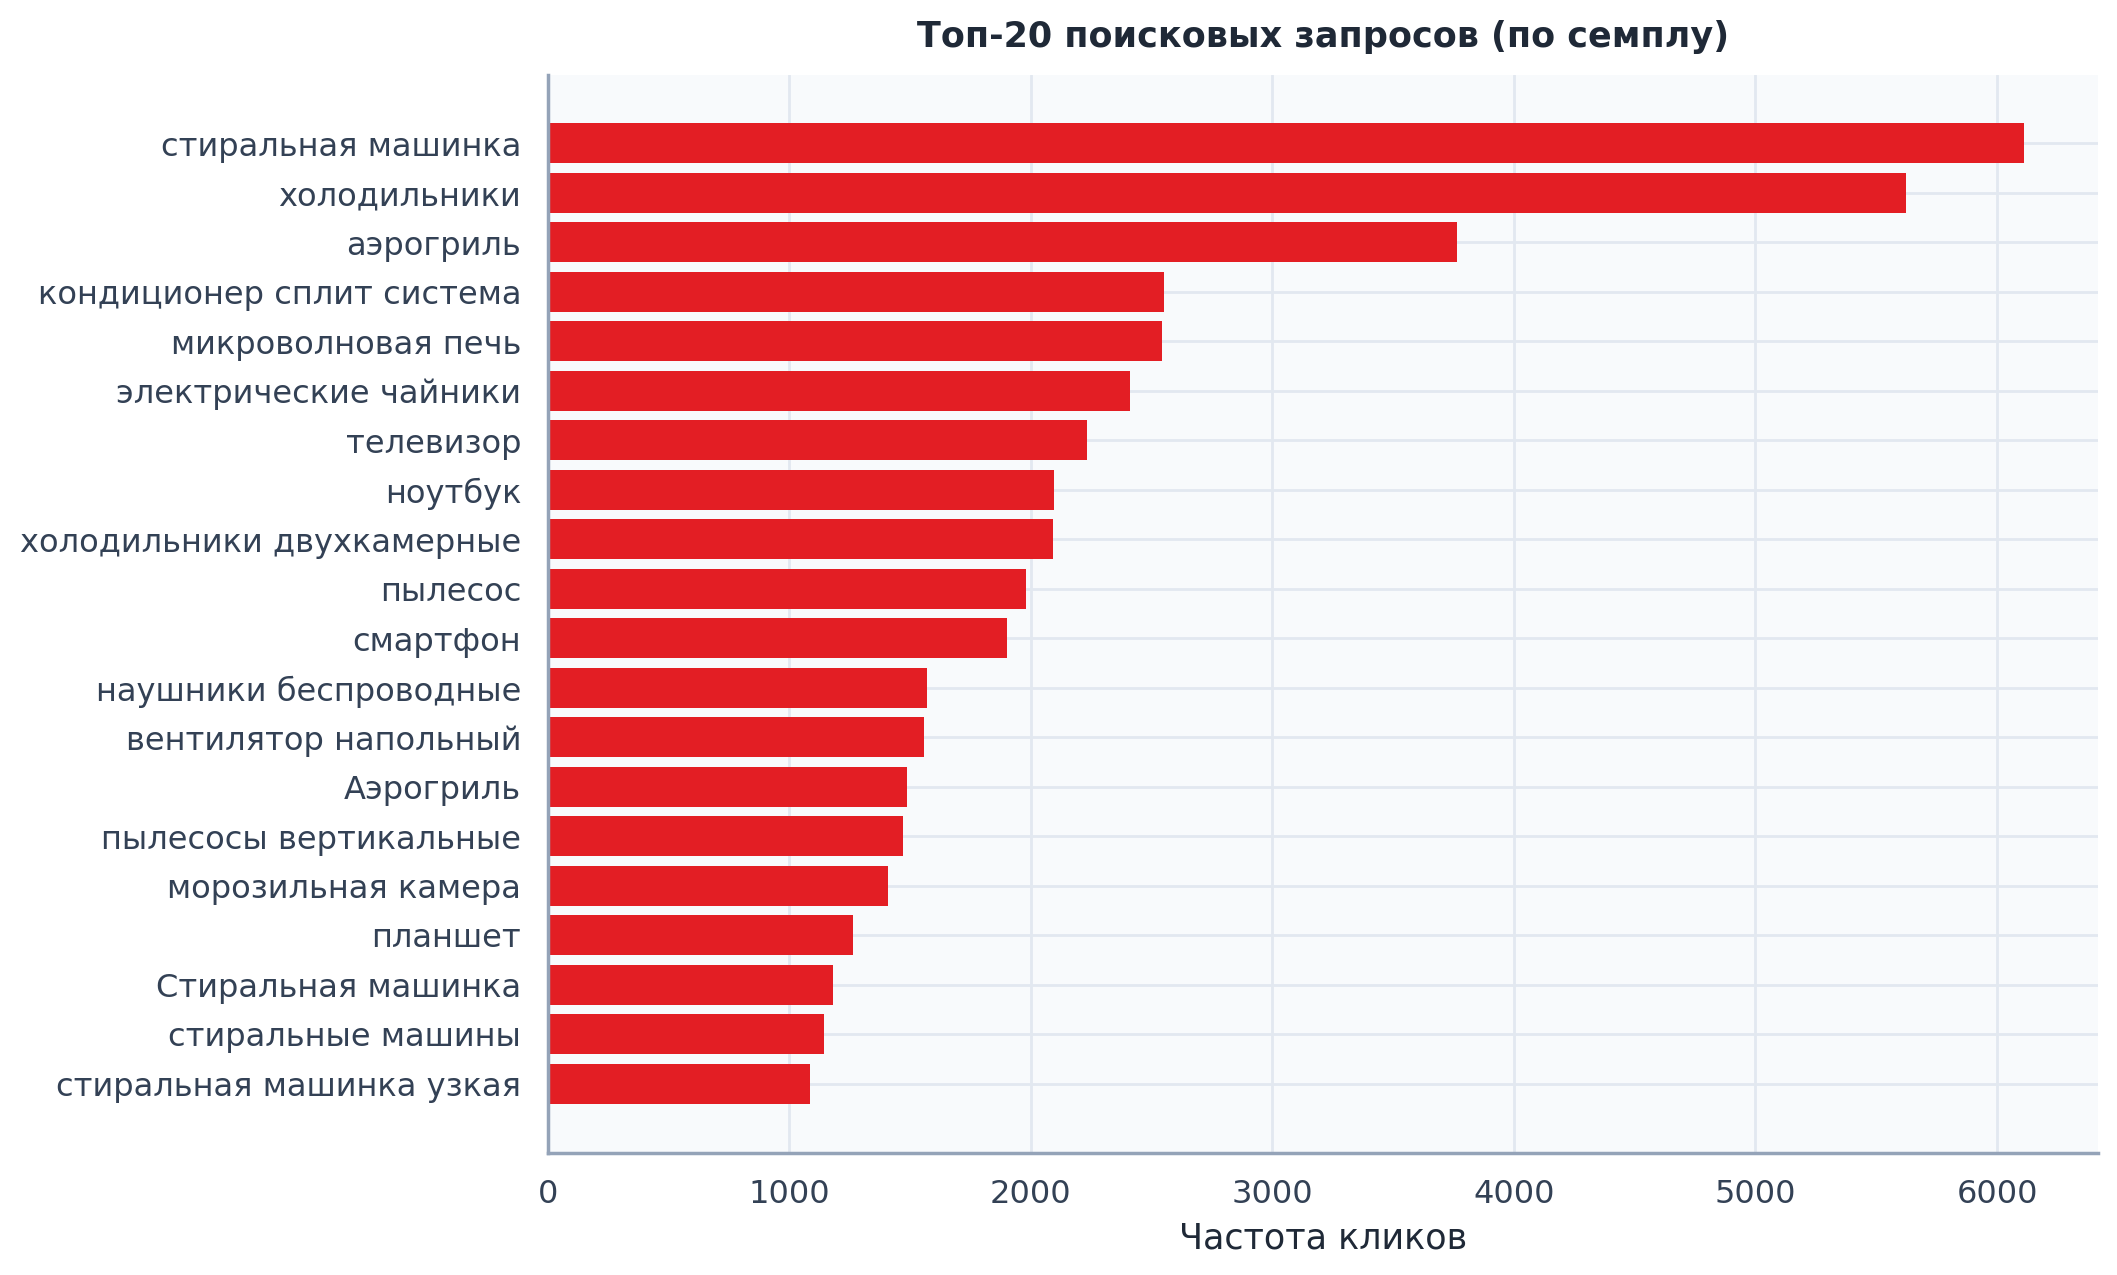
\includegraphics[width=0.92\textwidth]{figures/02_top_queries.png}}{\fbox{figures/02\_top\_queries.png}}
\caption{Топ поисковых запросов по кликам}
\end{figure}

\begin{figure}[H]
\centering
\IfFileExists{figures/03_top_brands.png}{
\includegraphics[width=0.92\textwidth]{figures/03_top_brands.png}}{\fbox{figures/03\_top\_brands.png}}
\caption{Топ брендов}
\end{figure}

\begin{figure}[H]
\centering
\IfFileExists{figures/01_query_length_dist.png}{
\includegraphics[width=0.85\textwidth]{figures/01_query_length_dist.png}}{\fbox{01}}
\caption{Распределение длины запросов}
\end{figure}

\begin{figure}[H]
\centering
\IfFileExists{figures/04_price_distribution.png}{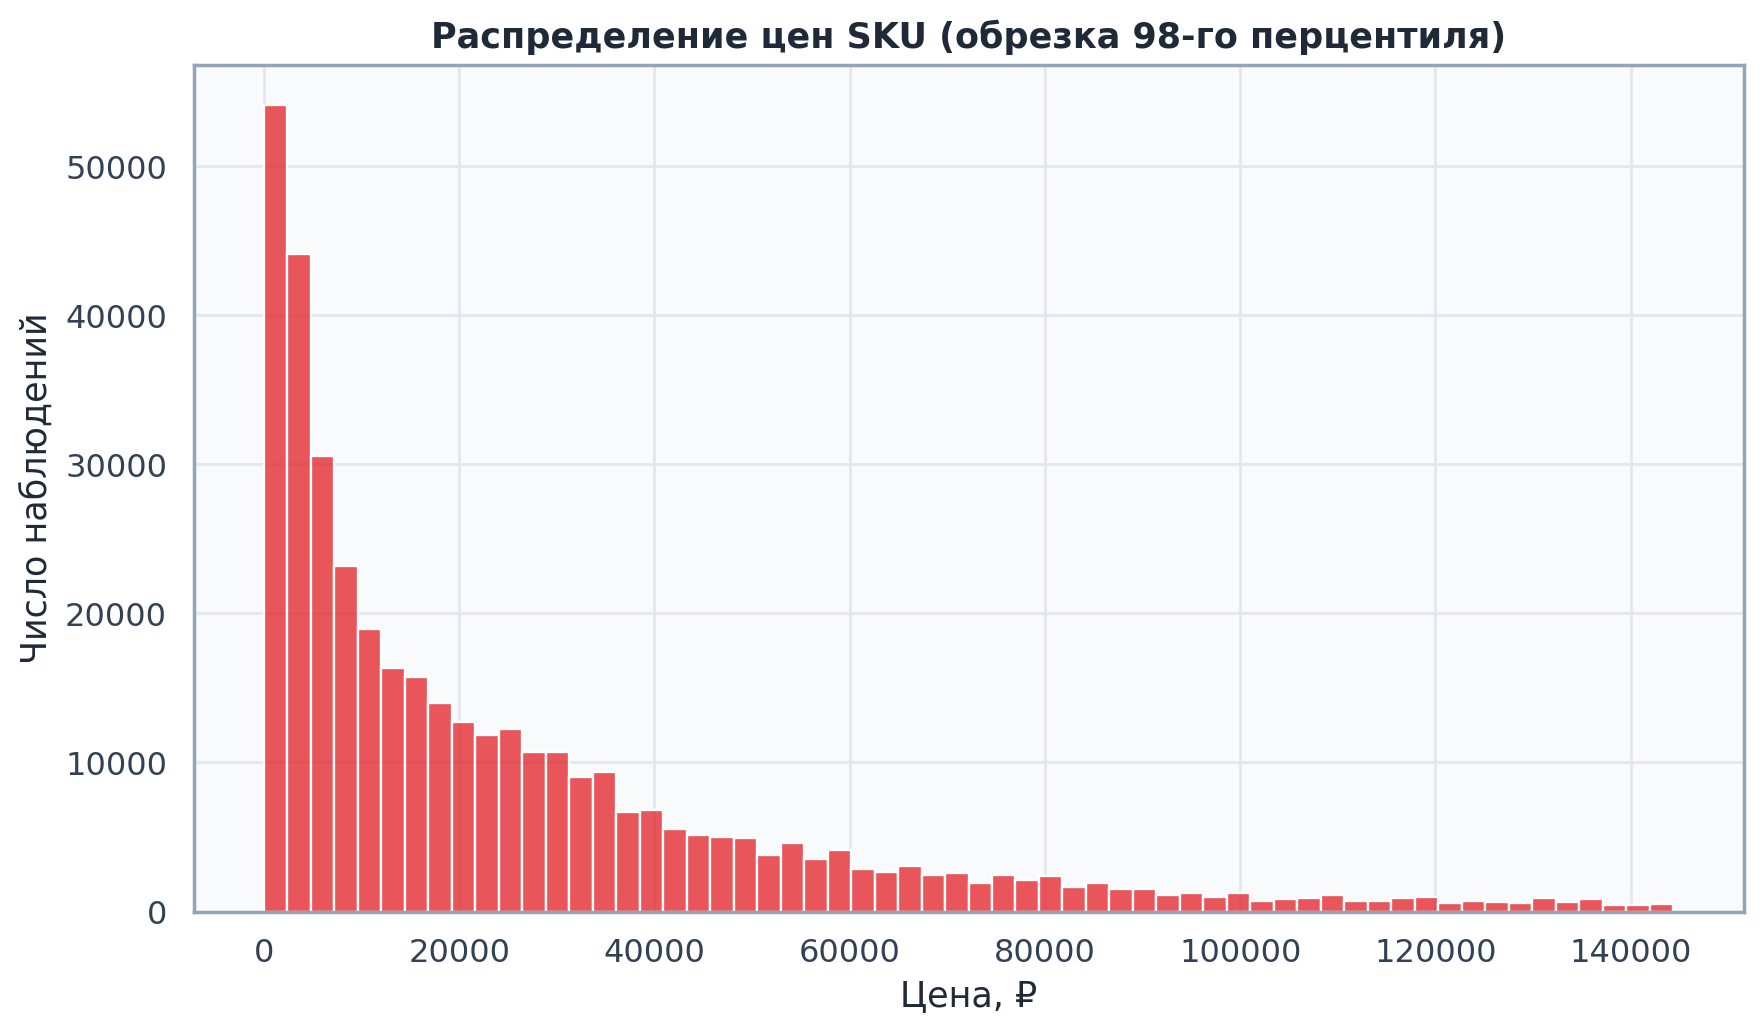
\includegraphics[width=0.85\textwidth]{figures/04_price_distribution.png}}{\fbox{04}}
\caption{Распределение цен кликнутых SKU}
\end{figure}

\begin{figure}[H]
\centering
\IfFileExists{figures/05_position_distribution.png}{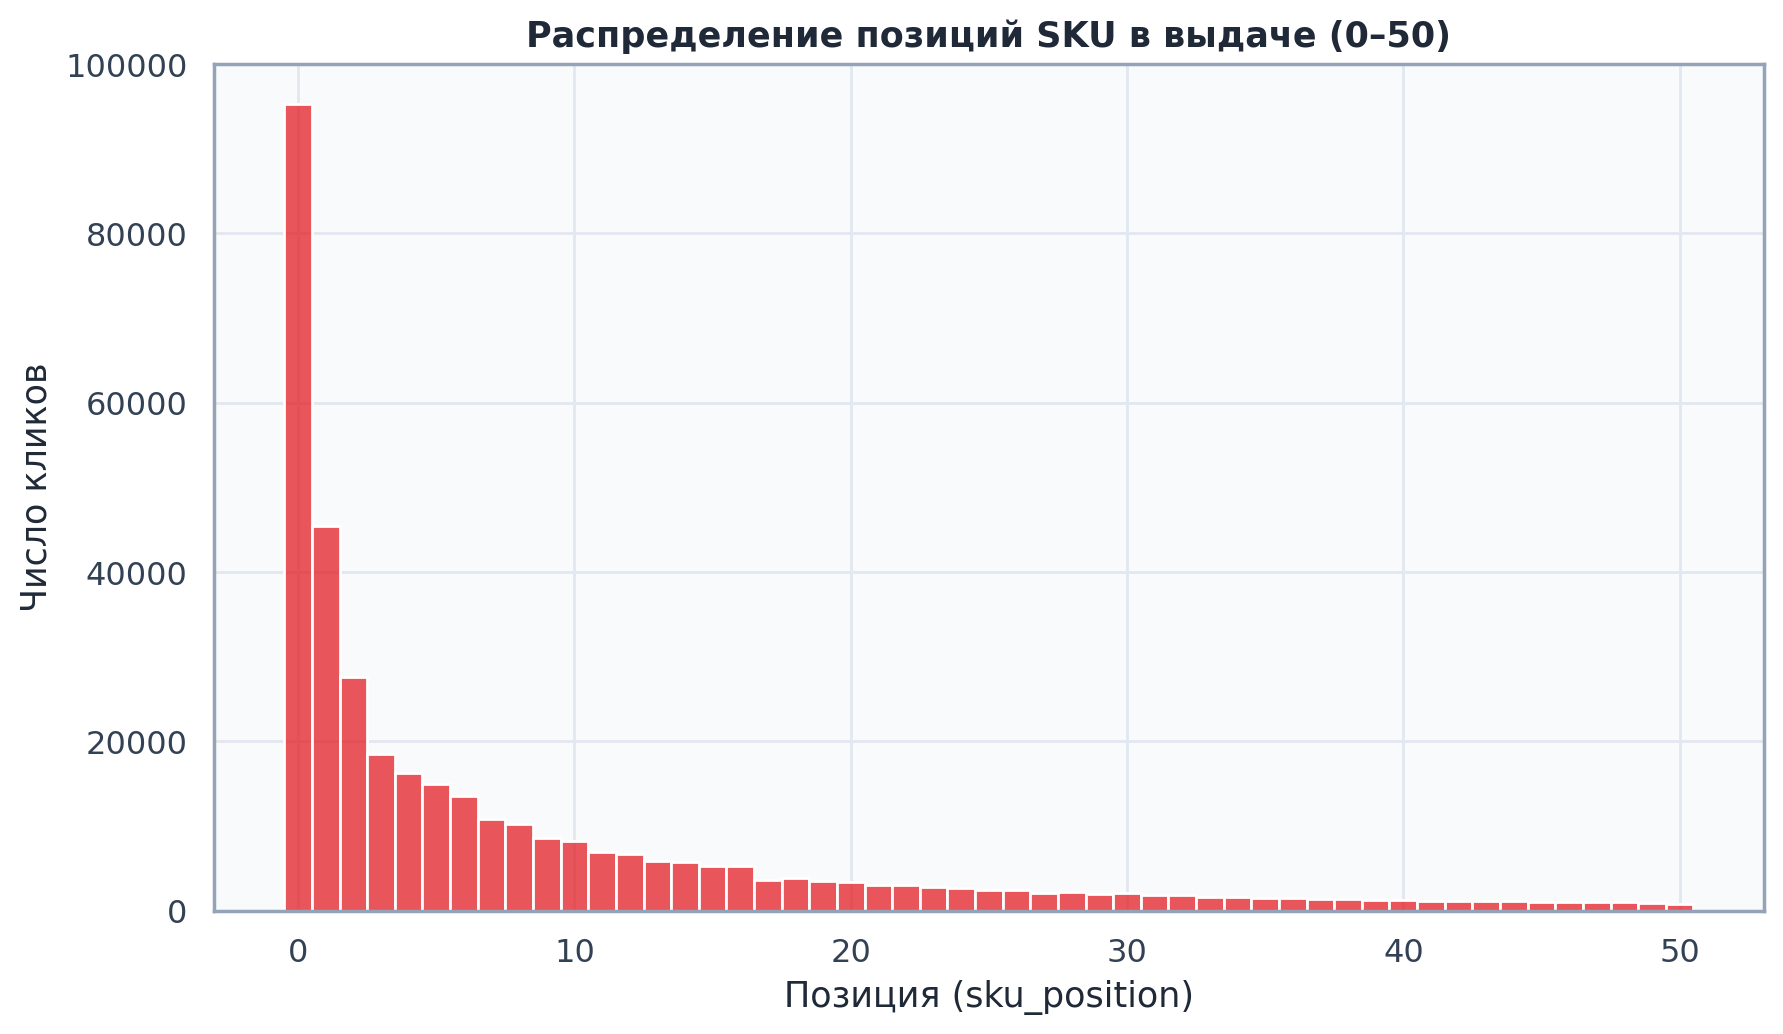
\includegraphics[width=0.85\textwidth]{figures/05_position_distribution.png}}{\fbox{05}}
\caption{Позиция SKU при клике}
\end{figure}

\begin{figure}[H]
\centering
\IfFileExists{figures/06_query_brand_heatmap.png}{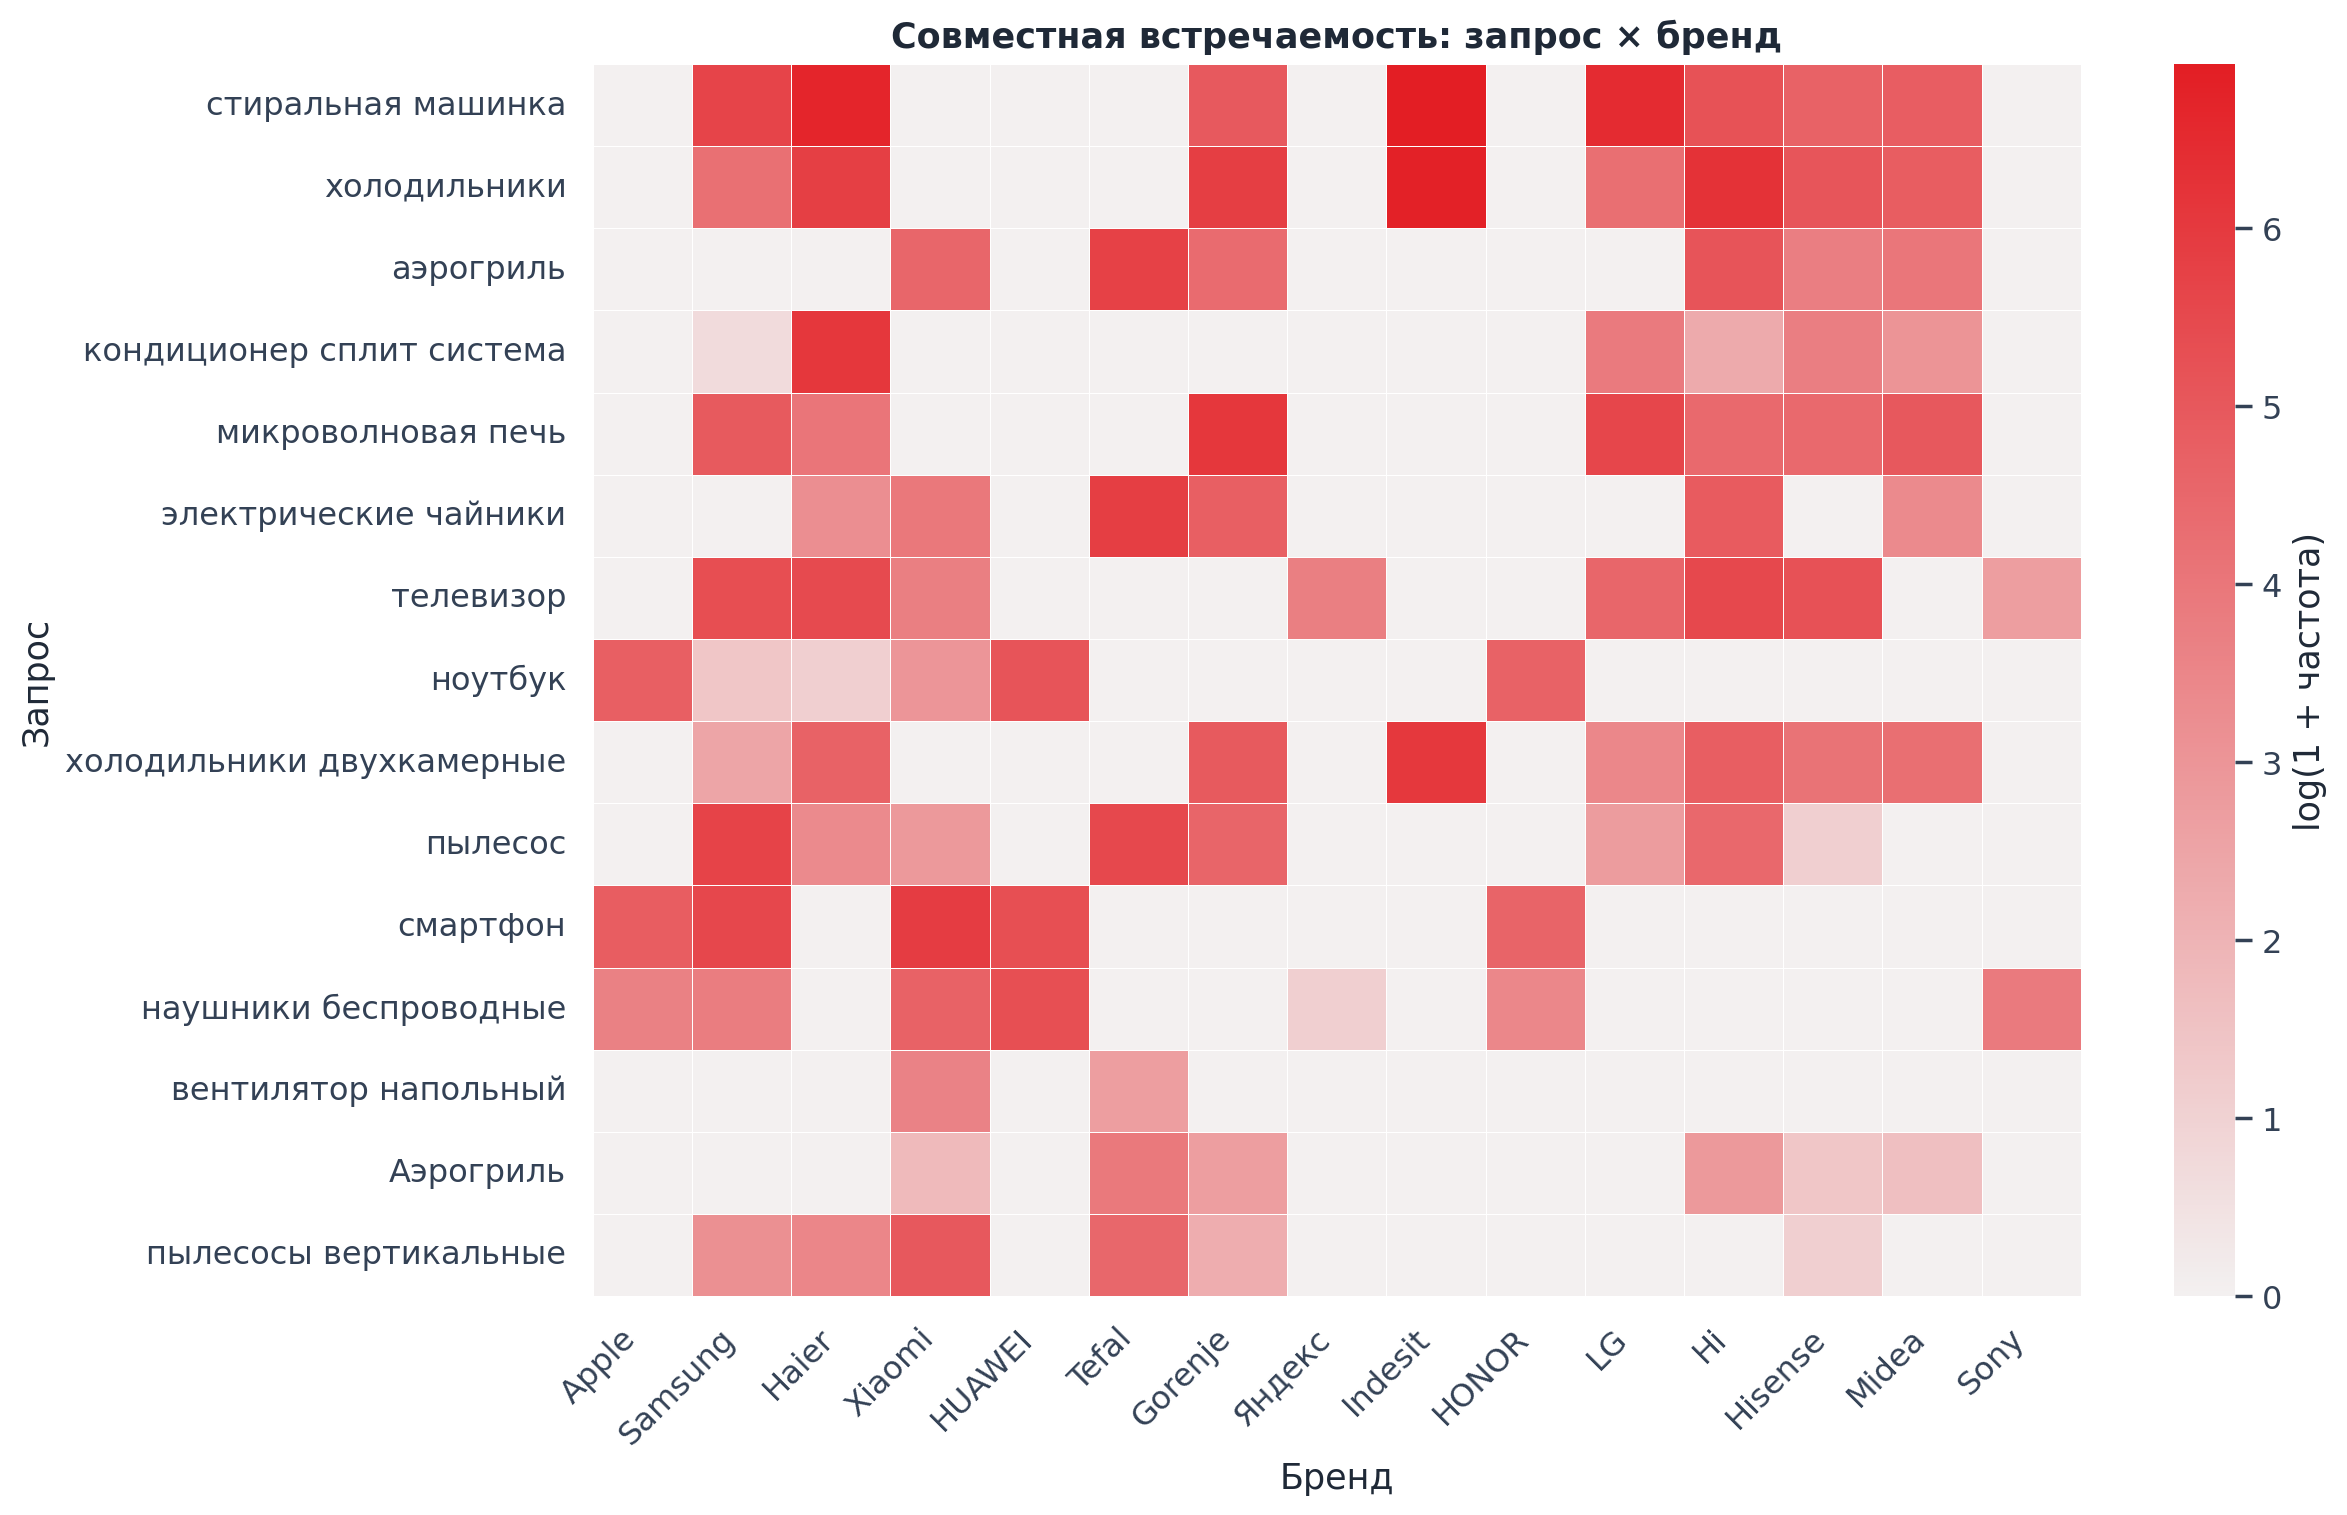
\includegraphics[width=0.95\textwidth]{figures/06_query_brand_heatmap.png}}{\fbox{06}}
\caption{Co-occurrence: запрос $\times$ бренд}
\end{figure}

\begin{figure}[H]
\centering
\IfFileExists{figures/07_tfidf_similarity_heatmap.png}{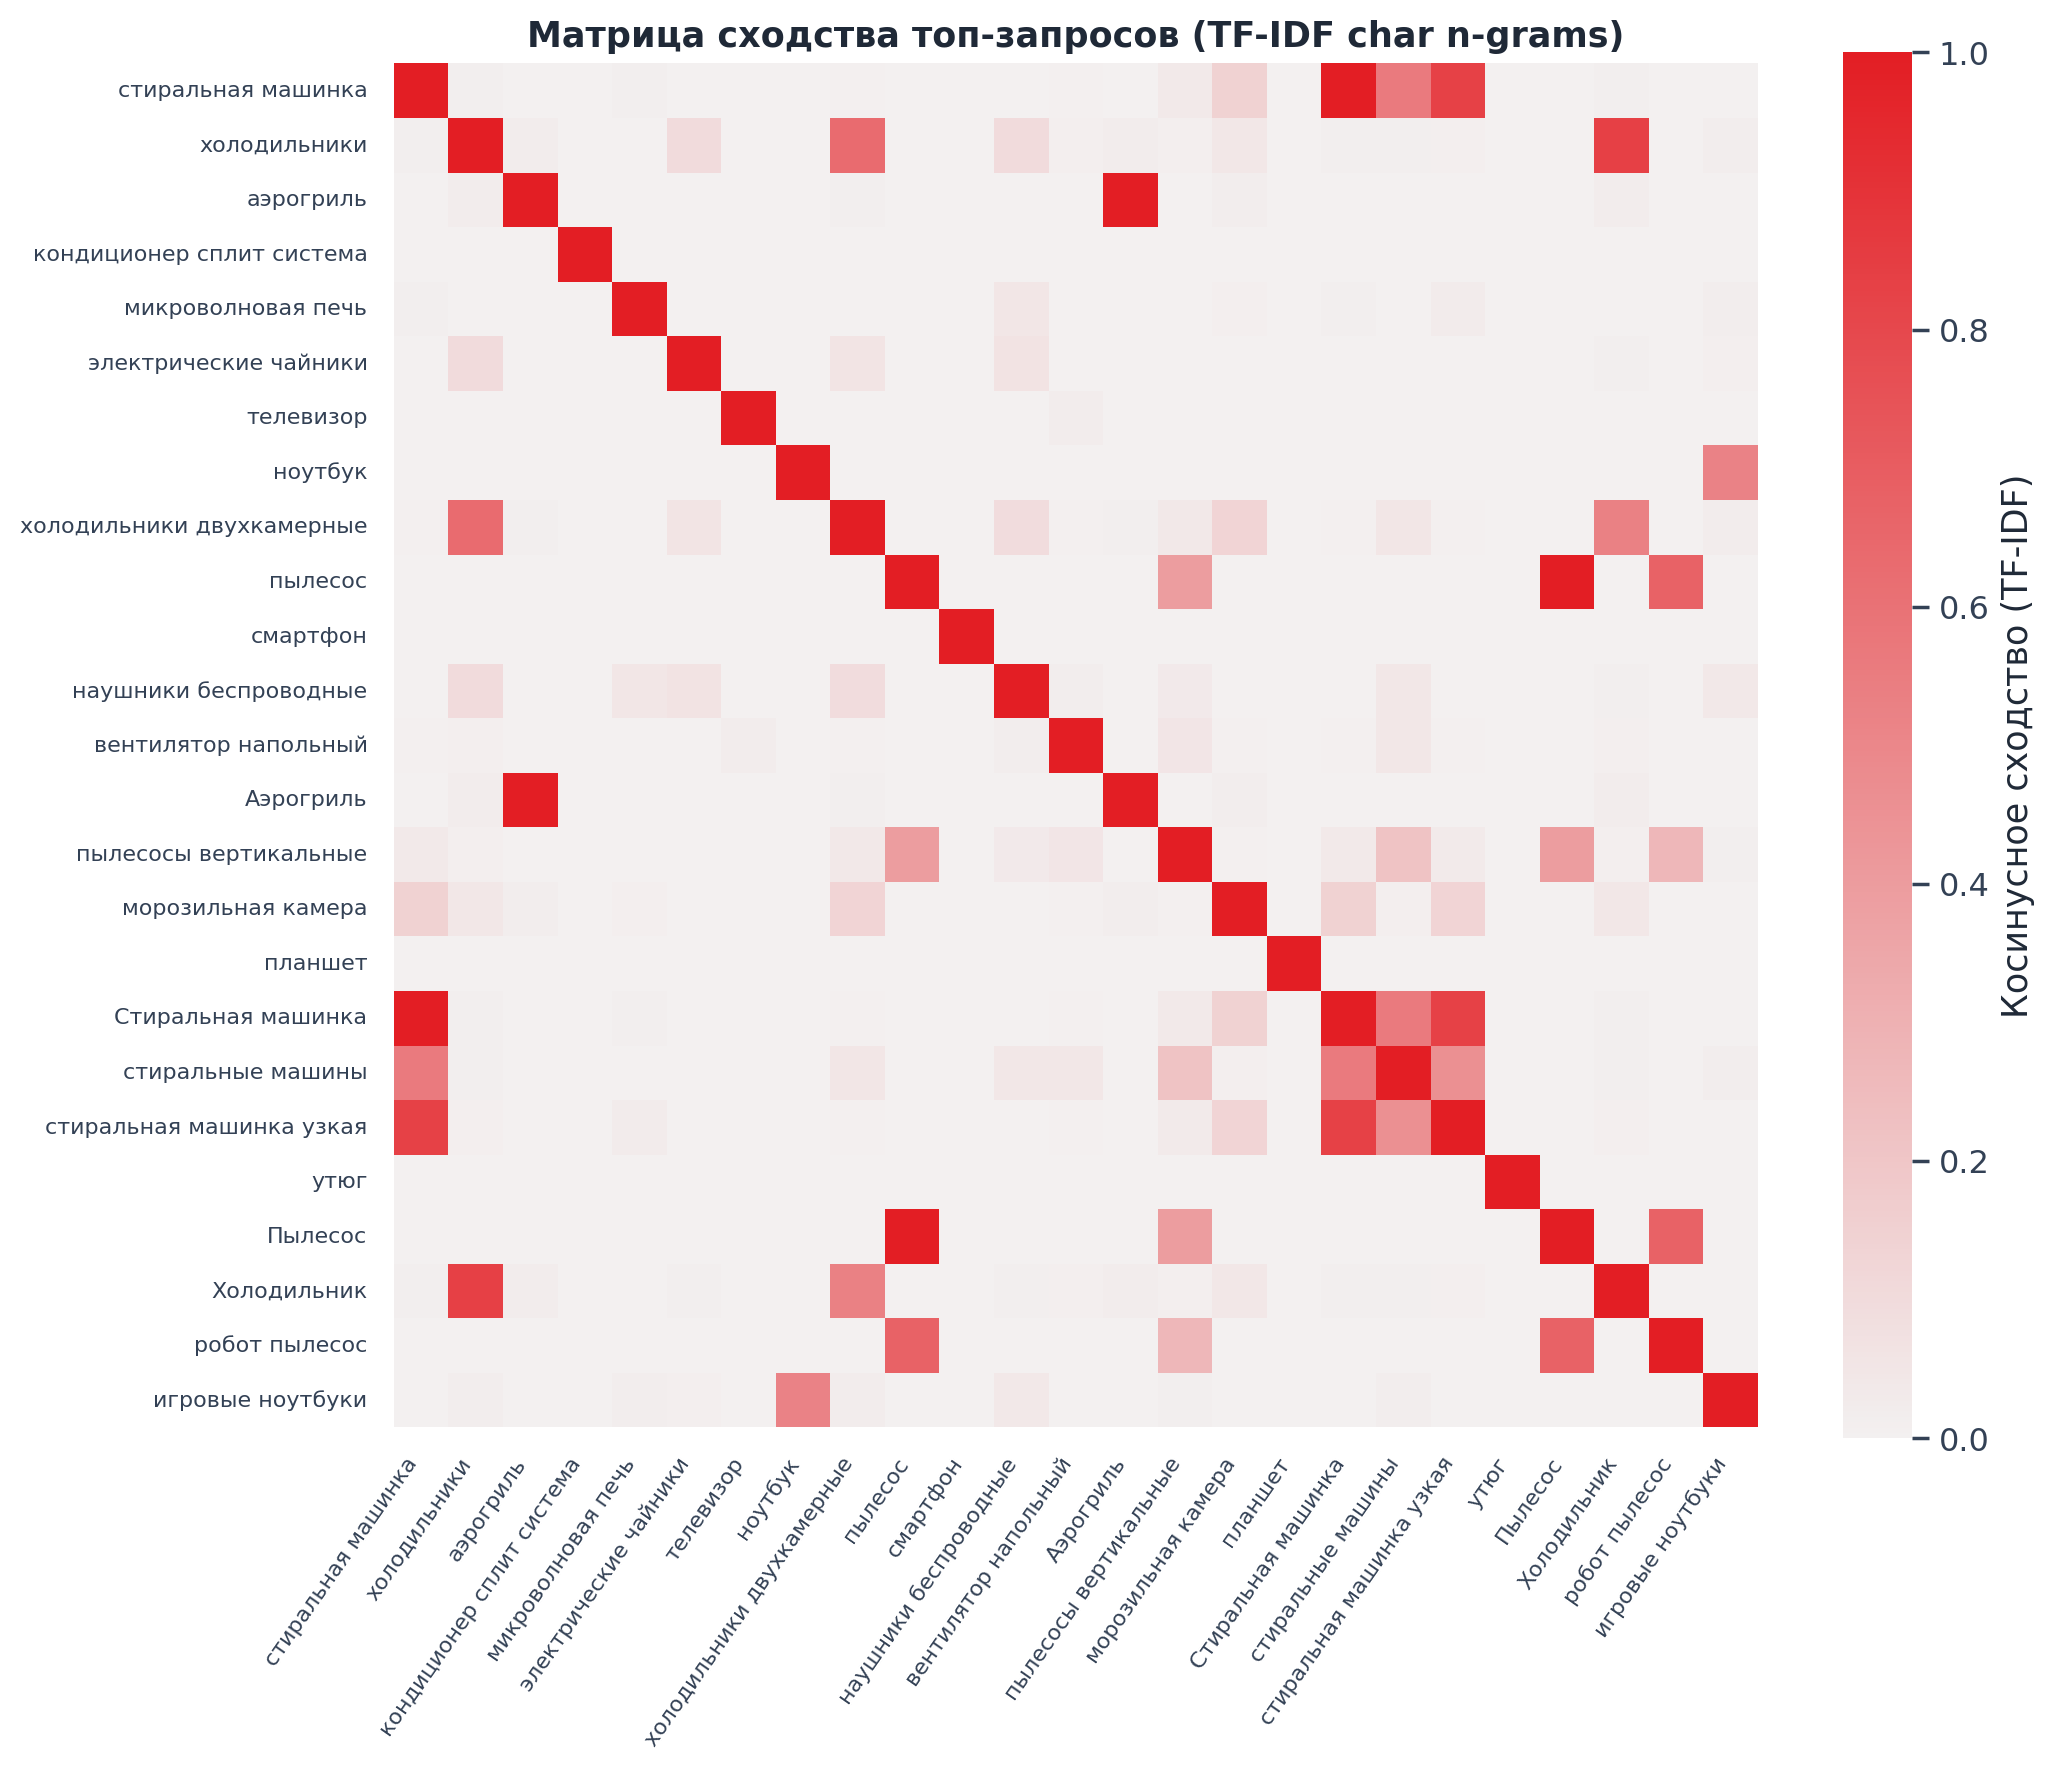
\includegraphics[width=0.95\textwidth]{figures/07_tfidf_similarity_heatmap.png}}{\fbox{07}}
\caption{Матрица косинусной близости TF-IDF запросов}
\end{figure}

\begin{figure}[H]
\centering
\IfFileExists{figures/10_price_vs_position.png}{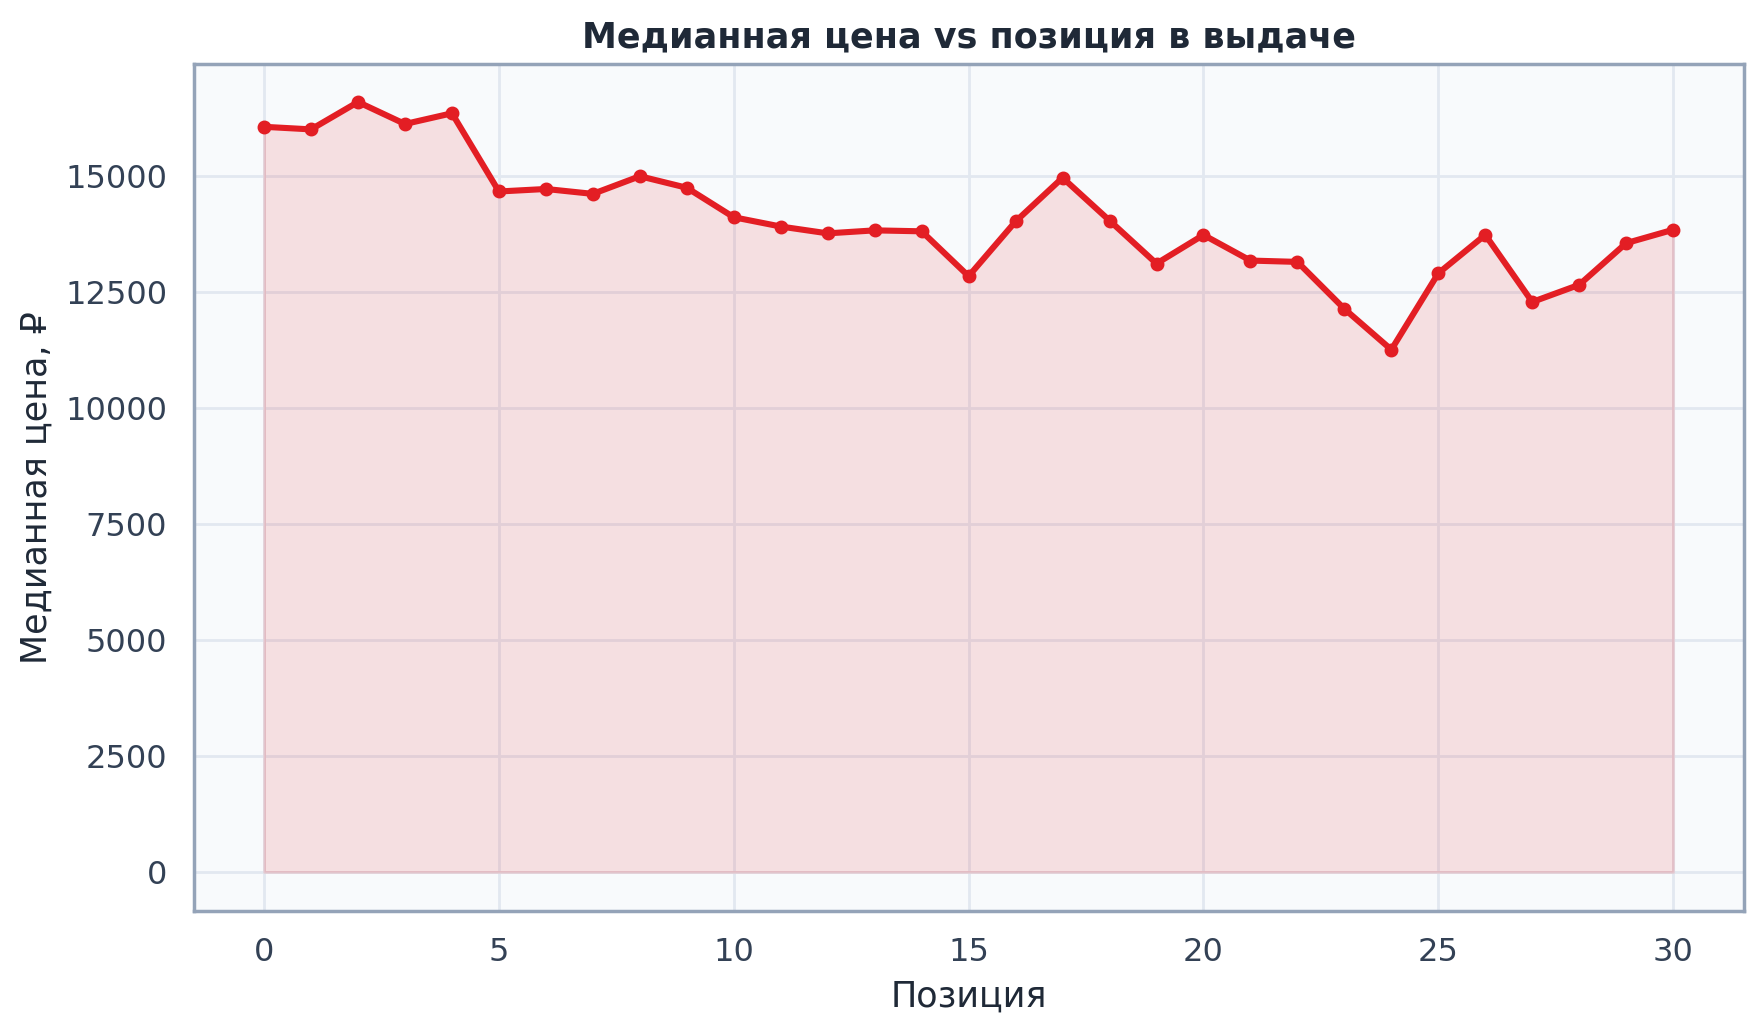
\includegraphics[width=0.9\textwidth]{figures/10_price_vs_position.png}}{\fbox{10}}
\caption{Цена vs позиция в выдаче}
\end{figure}

\newpage

\section{Методология}

\subsection{Слабая разметка (weak supervision)}

Из кликовых данных строятся словари брендов и категорийных фраз. По ним запросы размечаются в BIO-схеме с типами:
\begin{itemize}
    \item \cred{BRAND} --- бренд (Apple, Samsung, \ldots);
    \item \cblue{CATEGORY} --- тип товара (ноутбук, холодильник, \ldots);
    \item \cgreen{ATTR} --- характеристики (256~ГБ, OLED, цвет, диагональ).
\end{itemize}

\subsection{Модели}

\begin{purplebox}[Средняя сложность --- гибрид]
\begin{enumerate}
    \item \textbf{Baseline:} TF-IDF (char $n$-grams) + Logistic Regression $\to$ бренд по запросу.
    \item \textbf{NER:} CRF (\texttt{sklearn-crfsuite}) на орфографических и контекстных признаках токена.
    \item \textbf{Инференс:} словарь (exact) + RapidFuzz (fuzzy brand) + CRF $\to$ JSON.
\end{enumerate}
\end{purplebox}

Подход опирается на классические идеи курса ИИ: векторные представления текста, модели последовательностей, метрики классификации/NER, оптимизация latency для продакшн-сервиса.

\subsection{Формат ответа}

\begin{verbatim}
POST /extract
{"query": "смартфон apple 256"}

-> {
  "query": "...",
  "entities": [{"text":"apple","label":"BRAND", ...}],
  "brand": "Apple",
  "category": "смартфон",
  "attributes": {"256": "ATTR"},
  "latency_ms": 2.1
}
\end{verbatim}

\newpage

\section{Результаты и метрики}

Актуальные числа сохраняются в \texttt{artifacts/metrics.json} после запуска пайплайна.

\begin{figure}[H]
\centering
\IfFileExists{figures/18_metrics_summary.png}{
\includegraphics[width=0.98\textwidth]{figures/18_metrics_summary.png}}{\fbox{18}}
\caption{Сводка метрик: classifier / NER / latency}
\end{figure}

\begin{figure}[H]
\centering
\IfFileExists{figures/13_confusion_matrix.png}{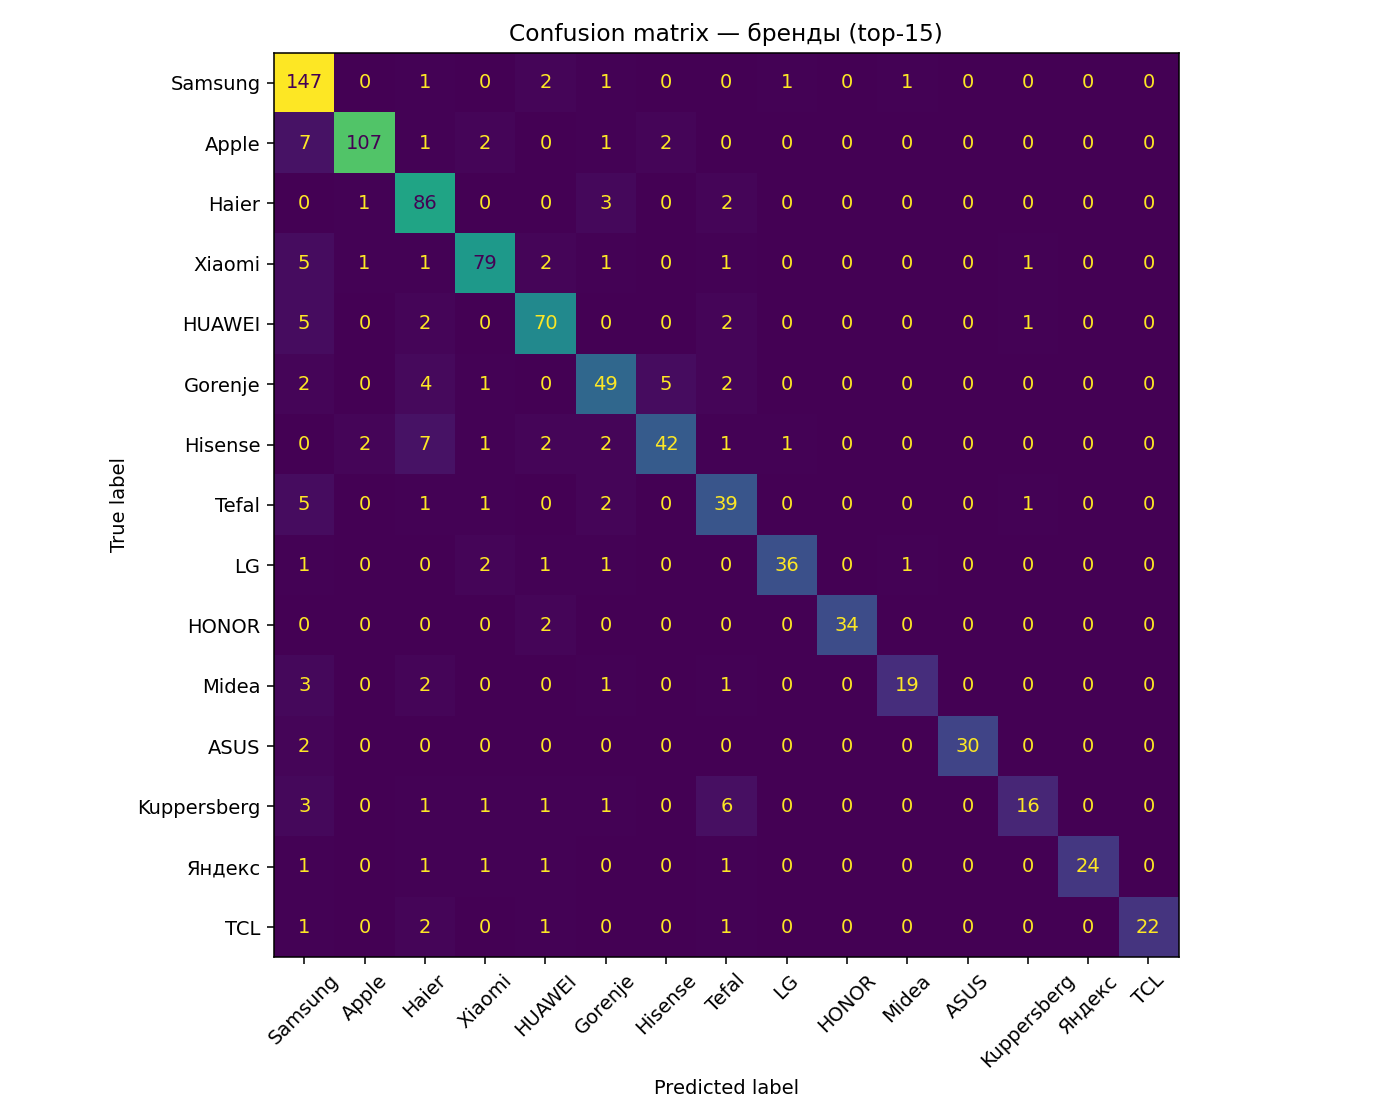
\includegraphics[width=0.88\textwidth]{figures/13_confusion_matrix.png}}{\fbox{13}}
\caption{Confusion matrix предсказания бренда}
\end{figure}

\begin{figure}[H]
\centering
\IfFileExists{figures/14_ner_f1_by_entity.png}{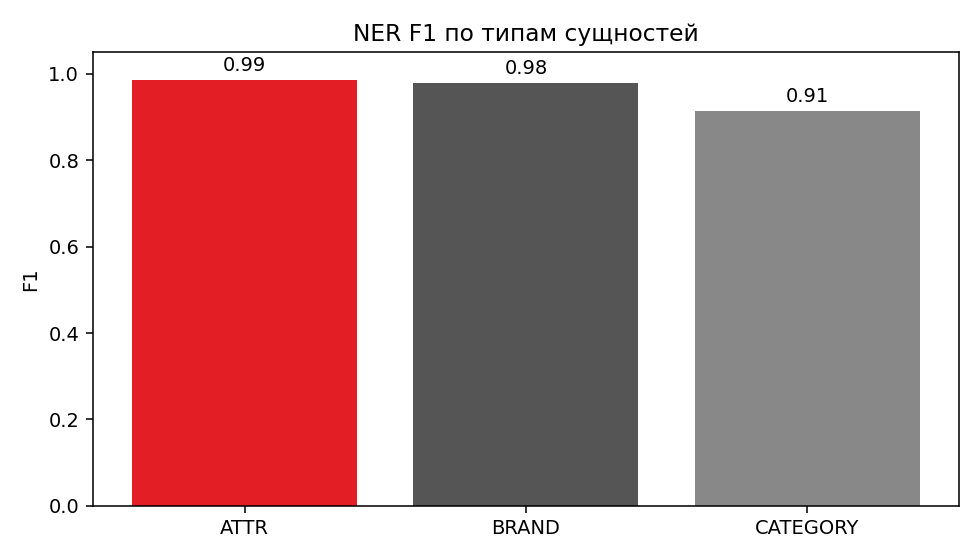
\includegraphics[width=0.75\textwidth]{figures/14_ner_f1_by_entity.png}}{\fbox{14}}
\caption{Entity F1 по типам сущностей}
\end{figure}

\begin{figure}[H]
\centering
\IfFileExists{figures/15_learning_curve.png}{
\includegraphics[width=0.8\textwidth]{figures/15_learning_curve.png}}{\fbox{15}}
\caption{Learning curve CRF NER}
\end{figure}

\begin{figure}[H]
\centering
\IfFileExists{figures/16_embedding_tsne.png}{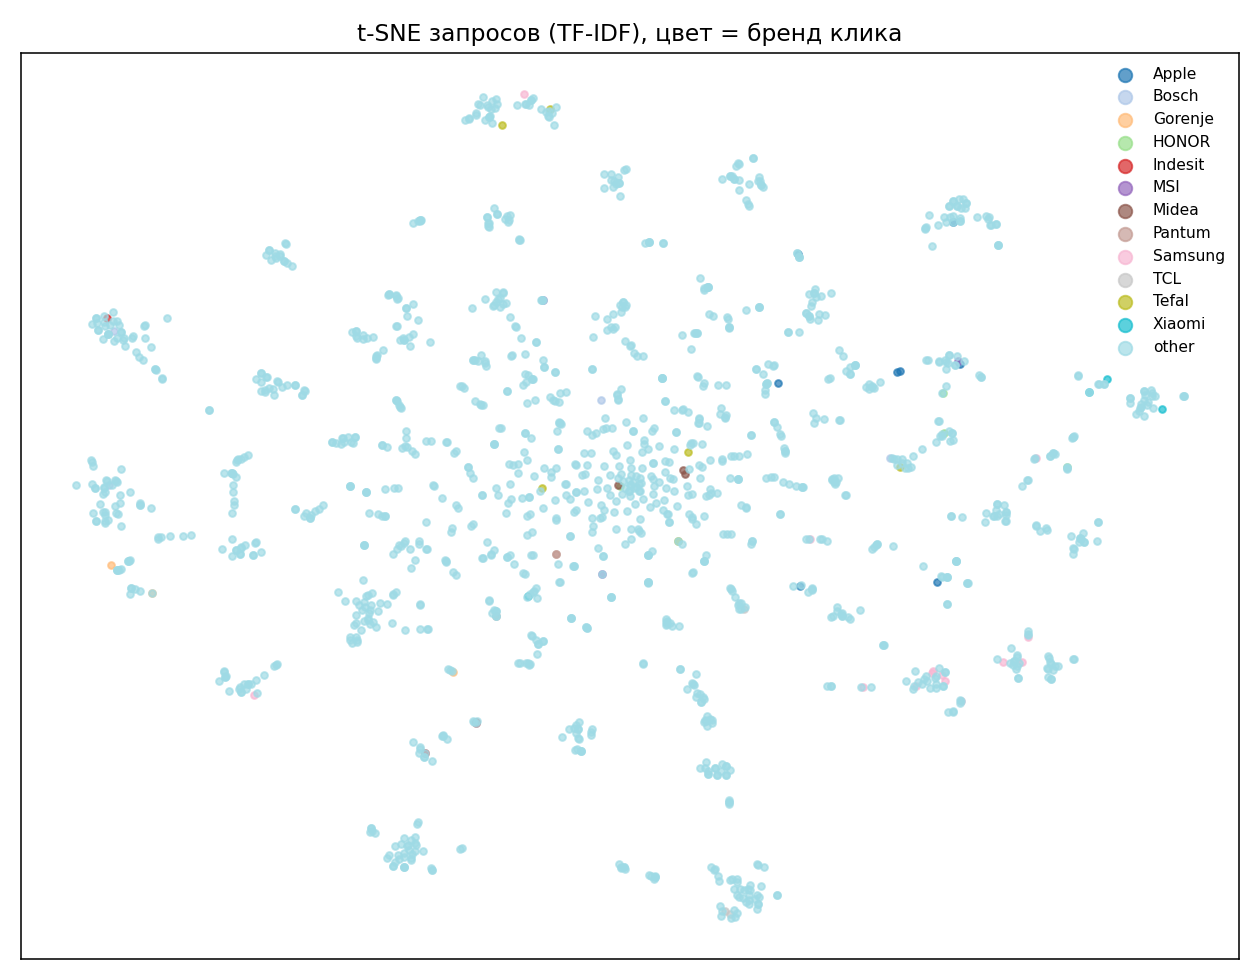
\includegraphics[width=0.8\textwidth]{figures/16_embedding_tsne.png}}{\fbox{16}}
\caption{t-SNE проекция запросов}
\end{figure}

\begin{figure}[H]
\centering
\IfFileExists{figures/17_latency_histogram.png}{
\includegraphics[width=0.85\textwidth]{figures/17_latency_histogram.png}}{\fbox{17}}
\caption{Гистограмма latency инференса}
\end{figure}

\begin{importantbox}[SLA]
Целевой порог --- 100~мс. Гибридный словарь+CRF на CPU обычно укладывается в единицы миллисекунд (см.\ p50/p95 в \texttt{metrics.json}).
\end{importantbox}

\newpage

\section{Структура репозитория}

\begin{table}[H]
\centering
\begin{tabular}{@{}p{4.2cm}p{10cm}@{}}
\toprule
\textbf{Путь} & \textbf{Назначение} \\
\midrule
\texttt{notebooks/01--12\_*.ipynb} & EDA, схожести, NER, сервис, демо \\
\texttt{scripts/run\_pipeline.py} & Полный прогон: графики + обучение + метрики \\
\texttt{src/ner/} & Разметка, признаки, CRF, extractor \\
\texttt{src/service/app.py} & FastAPI \texttt{/extract} \\
\texttt{figures/} & PNG-визуализации ($>$10) \\
\texttt{artifacts/} & Словари, \texttt{metrics.json} \\
\texttt{models/} & \texttt{crf\_ner.pkl}, baseline joblib \\
\texttt{docs/} & Эта LaTeX-документация \\
\texttt{файлы/} & Сырые данные (не в git) \\
\bottomrule
\end{tabular}
\end{table}

\subsection{Ноутбуки}

\begin{enumerate}
    \item \texttt{01\_data\_overview} --- схемы и размеры;
    \item \texttt{02\_eda\_queries} --- запросы;
    \item \texttt{03\_eda\_products} --- товары/бренды;
    \item \texttt{04\_similarity\_matrices} --- матрицы схожести;
    \item \texttt{05\_click\_patterns} --- клики и позиции;
    \item \texttt{06\_weak\_supervision\_ner} --- BIO-разметка;
    \item \texttt{07\_train\_baseline\_classifier} --- TF-IDF + LogReg;
    \item \texttt{08\_train\_ner\_model} --- CRF NER;
    \item \texttt{09\_embeddings\_similarity} --- эмбеддинги / t-SNE;
    \item \texttt{10\_service\_benchmark} --- latency;
    \item \texttt{11\_skus\_catalog\_explore} --- YML-каталог;
    \item \texttt{12\_end\_to\_end\_demo} --- демо JSON.
\end{enumerate}

\newpage

\section{Запуск}

\begin{summarybox}
\begin{verbatim}
pip install -r requirements.txt
python scripts/run_pipeline.py
uvicorn src.service.app:app --port 8000
\end{verbatim}
\end{summarybox}

\begin{remarkbox}[GitHub]
Репозиторий: \url{https://github.com/xWooshieL/mvideo-ner-search}.\\
Администратор-коллаборатор: \texttt{Nizier193}.
\end{remarkbox}

\section{Выводы и следующие шаги}

\begin{enumerate}
    \item Гибрид словарей и CRF даёт интерпретируемый и быстрый NER для e-commerce запросов.
    \item Weak supervision масштабируется на миллионы кликов без ручной разметки.
    \item Дальше: дообучение tiny-трансформера (RuBERT-tiny), нормализация опечаток, связка с ранжированием выдачи, онлайн A/B.
\end{enumerate}

\begin{figure}[H]
\centering
\IfFileExists{figures/19_similarity_queries.png}{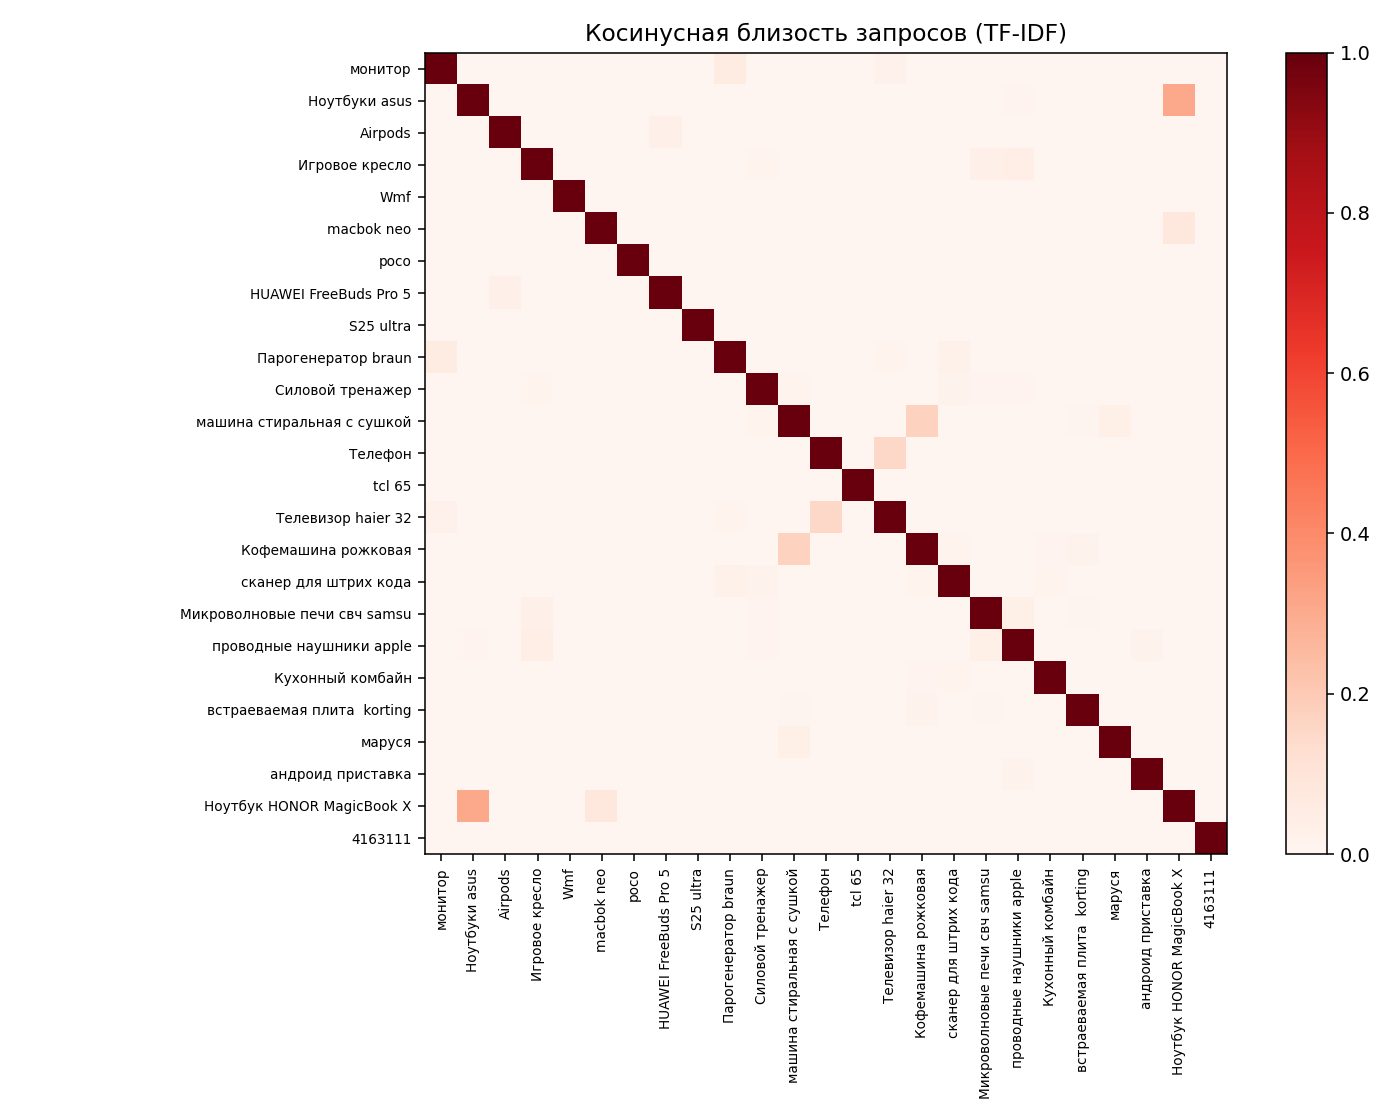
\includegraphics[width=0.85\textwidth]{figures/19_similarity_queries.png}}{\fbox{19}}
\caption{Доп.\ матрица схожести запросов}
\end{figure}

\begin{figure}[H]
\centering
\IfFileExists{figures/20_entity_distribution.png}{
\includegraphics[width=0.75\textwidth]{figures/20_entity_distribution.png}}{\fbox{20}}
\caption{Распределение сущностей в weak-labeled данных}
\end{figure}

\begin{figure}[H]
\centering
\IfFileExists{figures/12_brand_price_boxplot.png}{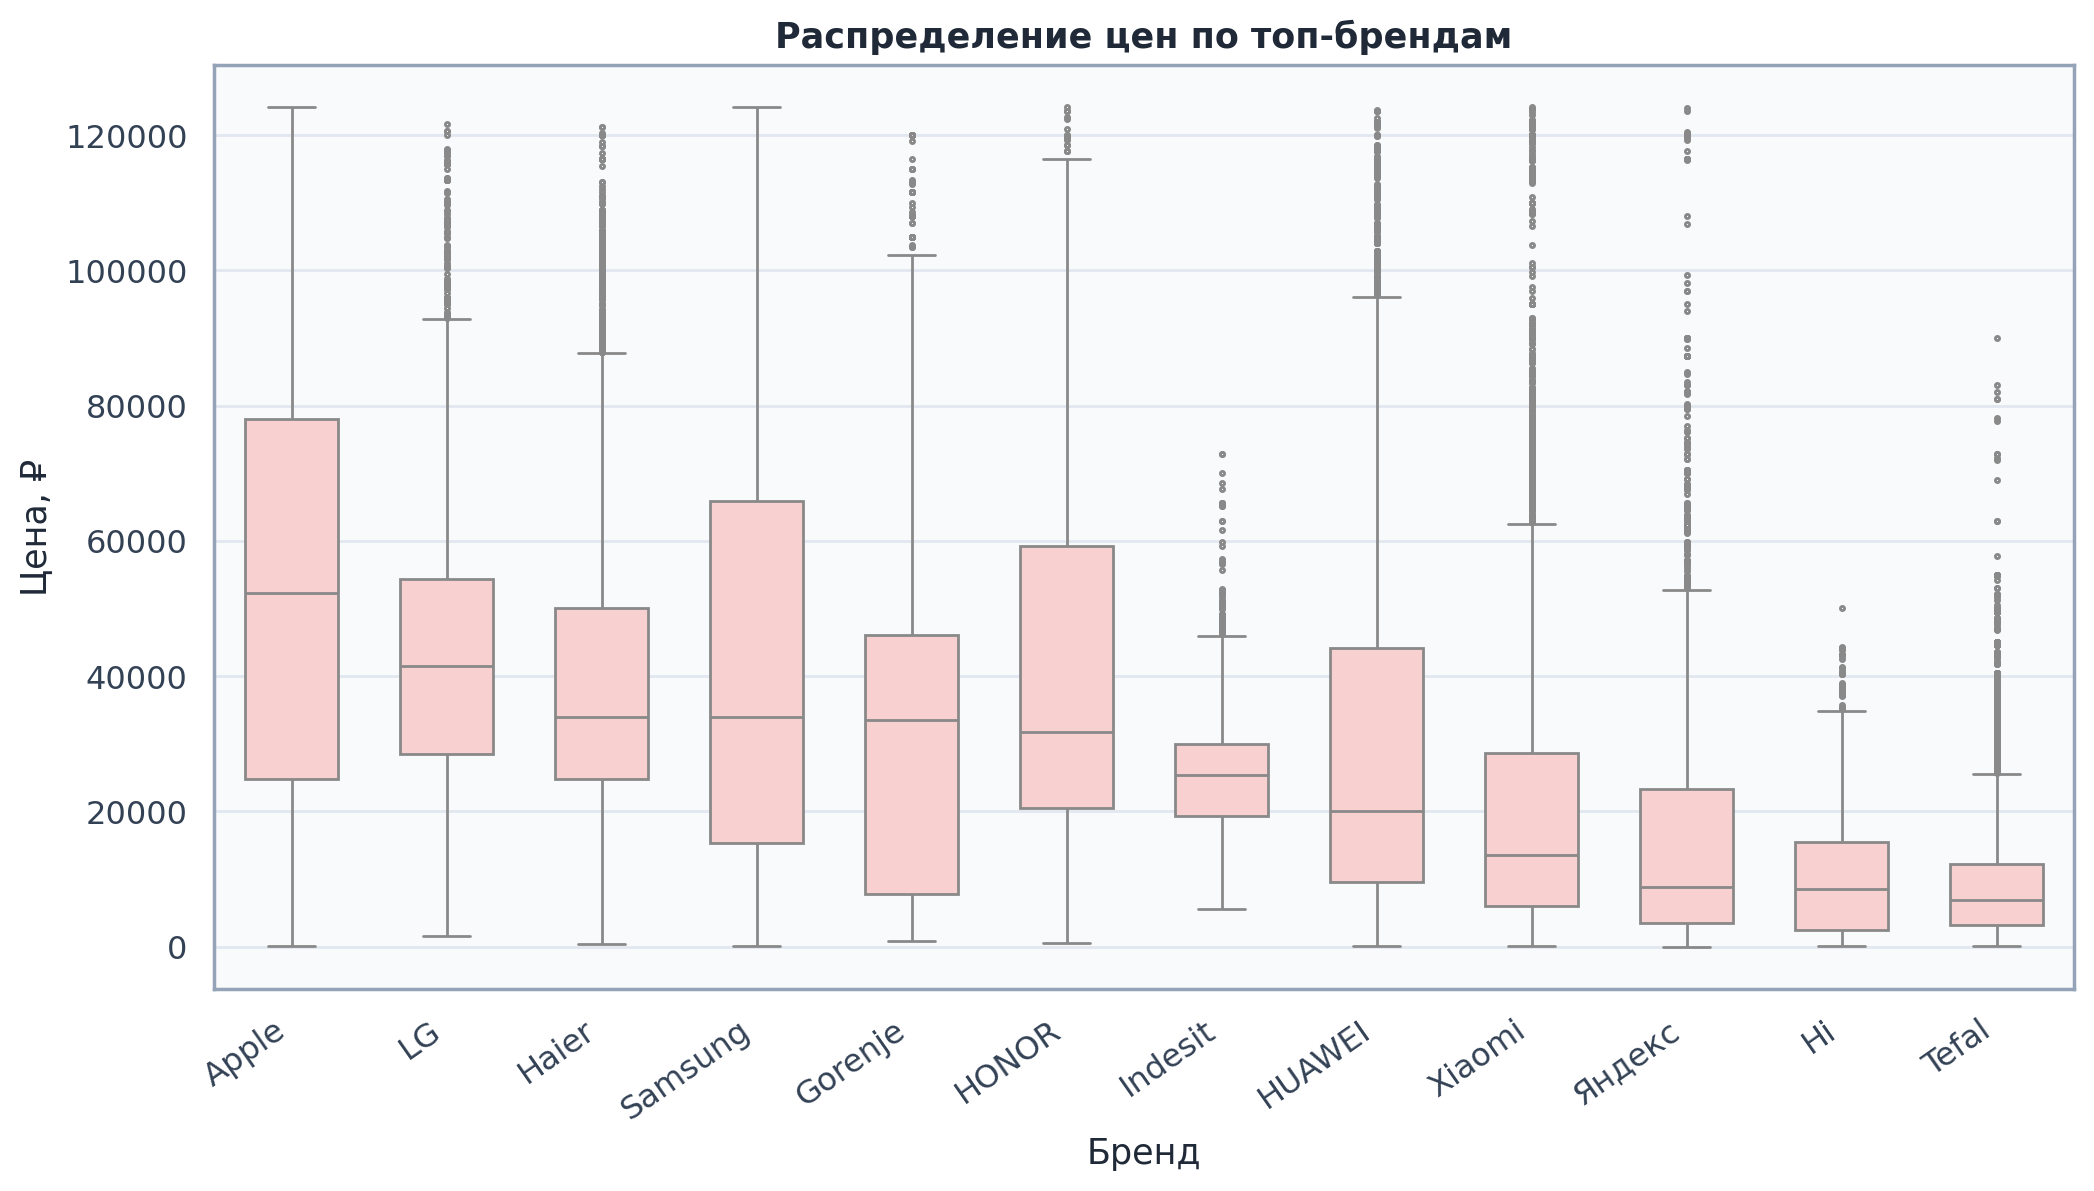
\includegraphics[width=0.9\textwidth]{figures/12_brand_price_boxplot.png}}{\fbox{12}}
\caption{Цены по топ-брендам}
\end{figure}

\vspace{1em}
\begin{center}
\textcolor{softgray}{\textit{Документация подготовлена для защиты кейса М.Видео --- буткемп ЦУ 2026}}
\end{center}

\end{document}
